\hypertarget{la-photographie-en-voyage-un-muxe9tier}{%
\section{La photographie en voyage, un métier
?}\label{la-photographie-en-voyage-un-muxe9tier}}
\emph{}
A l'approche du voyage, nous avons acheté un appareil photo. Un Canon
PowerShot G7X Mark II, vivement recommandé par Pierre.

\begin{figure}
\centering
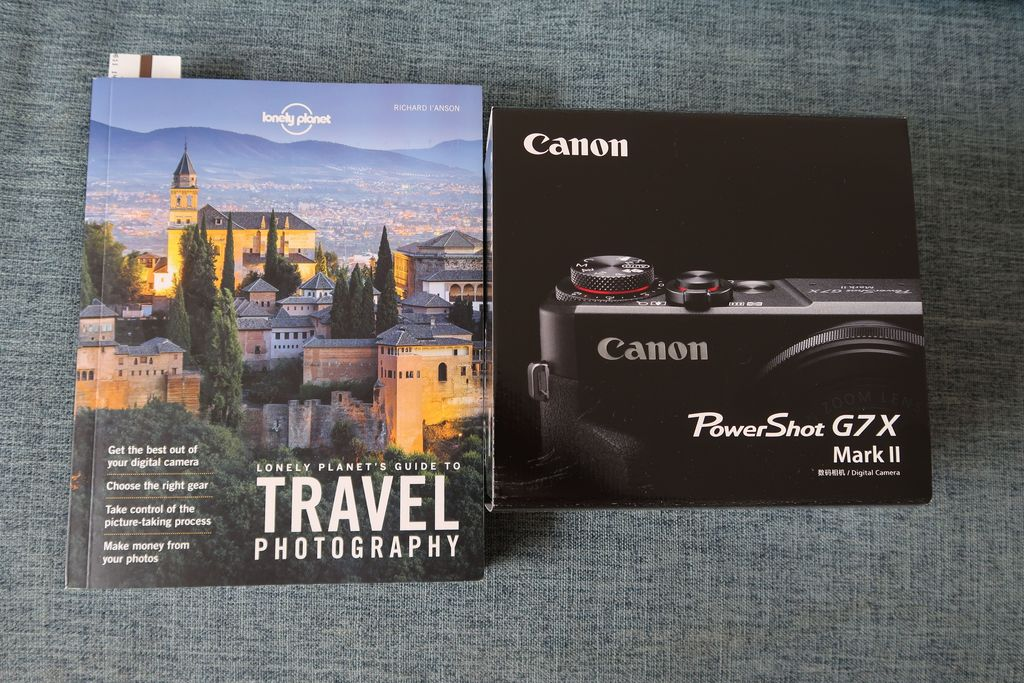
\includegraphics{images/appareil_photo_canon_g7x.JPG}
\caption{La boîte de l'appareil et le livre prêté par Ruocong pour
commencer à appréhender la thématique.}
\end{figure}

L'idée que je m'étais faite est que lorsqu'on est équipé d'un bon
appareil, on fait facilement des bonnes photos. Après quelques semaines
de pratique, je me rends bien compte que ce n'est que la partie émergée
de l'iceberg. On ne devient pas photographe en un jour.

Qu'à celà ne tienne, vous trouverez ci-dessous quelques exemples de
photos prises durant les dernières semaines avec ce bel appareil photo.
Ceci me permet également de tester l'intégration d'une gallerie photo
cliquable dans les articles de blog.

\emph{Florian}
